\documentclass[conference]{IEEEtran}
\IEEEoverridecommandlockouts
% The preceding line is only needed to identify funding in the first footnote. If that is unneeded, please comment it out.
\usepackage{comment}
\usepackage{pgfplots}
\usepackage{bib/paper_alcides}
\usepackage{cite}
\usepackage{amsmath,amssymb,amsfonts}
\usepackage{algorithmic}
\usepackage{graphicx}
\usepackage{textcomp}
\usepackage{xcolor}
\usepackage{adjustbox}
\def\BibTeX{{\rm B\kern-.05em{\sc i\kern-.025em b}\kern-.08em
    T\kern-.1667em\lower.7ex\hbox{E}\kern-.125emX}}
\begin{document}

\title{A Study in CUDA Usage}


\author{\IEEEauthorblockN{Pedro Carrega}
\IEEEauthorblockA{\textit{Departamento de Informática} \\ %devia ser em ingles?
\textit{Faculdade de Ciências da Universidade de Lisboa}\\
Lisboa, Portugal \\
fc49480@alunos.fc.ul.pt}
\and
\IEEEauthorblockN{Vasco Ferreira}
\IEEEauthorblockA{\textit{Departamento de Informática} \\ %devia ser em ingles?
\textit{Faculdade de Ciências da Universidade de Lisboa}\\
Lisboa, Portugal \\
fc49470@alunos.fc.ul.pt}
}

\maketitle

\begin{abstract}
This paper was developed with the purpose to explain GPU (Graphical Processing Unit) programing and the improvements that can be made. To demonstrate this we used the Floyd-Warshall algorithm since it is very demanding for the CPU (Central Processing Unit) due to the high number of computations required. During our research we discovered that the available materials for learning GPGPU (General Purpose Graphics Processing Unit) are quite difficult to understand for those who are looking to learn the basics of GPU programing. For that we developed this paper explaining from scratch GPGPU and some of the most significant improvements that can be made. We will start with a simple sequential solution of the algorithm in CUDA and from there go step by step till we use most of the tools and processing power that a GPU has to offer. This paper is helpful for someone who intends to learn the basics of GPGPU or could be used as a teaching guide in an IT course to introduce GPGPU to students.
\end{abstract}

\begin{IEEEkeywords}
GPGPU, CUDA, Floyd-Warshall.
\end{IEEEkeywords}

\section{Introduction}
The purpose of this paper is to teach GPU (Graphics Processing Unit) programing and the different improvements that can be made, showing the different improvements in each version so that the solution can perform even better taking advantage of the GPU optimizations. To demonstrate this, we used a well known problem that is the Floyd-Warshall algorithm. The algorithm calculates all the possible paths between two points and saves the shortest path. It was chosen because it requires a enormous amount of computation to get the final result since it is has O$(n^{3})$ complexity. With a high amount of entries, that is, a big matrix and so it can be very demanding for the CPU (Central Processing Unit). This is where the GPU benefits due to its high number of threads.
\newline
For this paper all the examples will be in CUDA. %outras linguagens tem estas coisas?

To make a method to be computed in the GPU you need to declare it with the "\_\_global\_\_" qualifier so that it will run on the GPU when called in the CPU. Each kernel runs a grid which is the group of blocks that are launched by the kernel, where each block is a set of threads. The grid can be represented as a one dimensional array, a two dimensional array or a three dimensional array. This can be used to improve the mapping of the work that each thread will do. 

When launching a kernel it has to be declared the number of threads per block and the number of blocks that are going to be used. It should be taken into consideration the fact that blocks are composed of warps which are a set of 32 threads, so when declaring the number of blocks being used, it should be a multiple of 32 since all threads in a warp use the same program counter. Therefor if the number of threads in the blocks is not multiple of 32 there will be threads that are busy, waiting for the other threads in their warp that are actually doing some work.

The composition of the kernel grid has a huge impact on performance, with that in mind a programmer of GPGPU (General Purpose Graphics Processing Unit), in most scenarios, should aim to use the largest amount of threads per block possible.

It also needs to be considered that the GPU does not have access to the memory used by the CPU, so all pointers used as input for the GPU kernel will have to be allocated and copied to the GPU global memory before being able to access it. The pointers of the memory that were allocated need to be passed through the parameters of the kernel call so that they can be used by the GPU. In case of a primitive type, it can be passed only by the parameters of the kernel (i.e. int) and does not need to allocate memory on the GPU memory manually. After all the computations are finished, the result should be accessible by the CPU so that it can copy back the result to the CPU and do what it needs with it. To do that it needs to copy the result similarly to the opposite operation but this time from the device to the host. Then the memory that was allocated in the GPU memory should be freed so there are no memory leaks just like in the CPU. In the next figure you can see an example of a input being copied to the GPU, the call of the kernel, the corresponding composition of the grid which will be represented in the (Fig.1) and then the result being copied back to the CPU memory:
\begin{lstlisting}[language=C++, caption=CUDA Example]
int* matrix_pointer_device;

cudaMalloc(&matrix_pointer_device, sizeof(int) * graph_sizeX * graph_sizeY);

cudaMemCpy(matrix_pointer_device, graph, sizeof(int) * graph_sizeX * graph_sizeY, cudaMemcpyHostToDevice);

dim3 threads(3,2);
dim3 blocks(4,2); 

computes<<<blocks, threads>>>(graph_sizeX, graph_sizeY, matrix_pointer_device);

cudaMemCpy(graph, matrix_pointer_device, sizeof(int) * graph_sizeX * graph_sizeY, cudaMemcpyDeviceToHost);

cudaFree(cudaMemcpyDeviceToHost);

\end{lstlisting}

\begin{figure}[htbp]
	\centerline{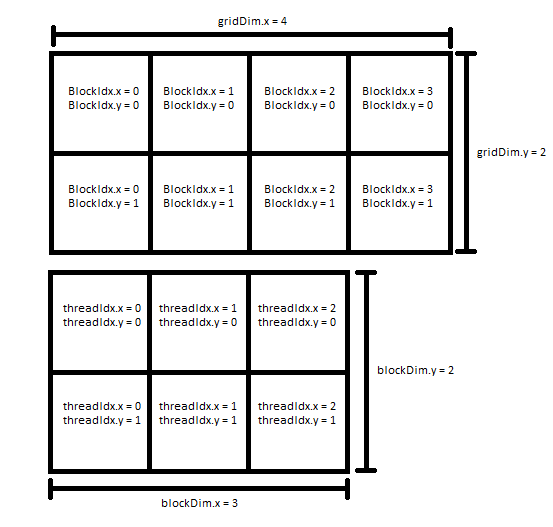
\includegraphics[width=\linewidth]{figures/gridExampleTransparant.png}}
	\caption{Example of a grid composition and block composition.}
	\label{fig1}
\end{figure}
\begin{comment}
	

\section{Background}

%how FW is computed
This is an optional section, as it depends on your project. In projects where a given specific knowledge is required to understand the article, you should give a brief introduction of the required concepts. In the case of genetic algorithms, you should present the basic algorithm in this section.


\section{Approach}


\end{comment}
\section{Implementation Details}

As said before, the grid can be 1D, 2D or 3D. Our approach was to use 1D, since if for example we used 2D, we would have to do the square route of the number of blocks per thread and the number of blocks in the grid. By doing so we would possibly be wasting some threads when both numbers are not perfect squares, by doing so then it would not be archived the best occupancy\cite{occupancy}.

Considering the average utilization of GPGPUs, the number of computations executed by a single program is enormous. The computation of one value per threads is not a realistic expectation, and such thread scheduling is something the user must consider. Thread scheduling carries a huge overhead to the computation and so it's something to be avoided if possible. With that in mind, we will be making so that each thread computes more than one result per call avoiding the need to rely on the GPU scheduler. 

To avoid scheduling it's required to correctly select the number of blocks and threads in each block. To help the user make said selection, CUDA provides multiple tools so that the user can select the most optimal number of blocks and threads per blocks. One exemple of said tools, and one used during the implementation of some of our solutions is "cudaOccupancyMaxPotentialBlockSize". Given the address of two integers, the amount of shared memory planed on using and the kernel call in question, the values of the integers are updated with the optimal number of blocks and threads per block. After that we calculated the work that each thread will do using the following formula:
\newline\newline
\centerline{workPerThread =$\frac{graph\_size^2}{blocksInGrid*threadsPerBlock}$}
\newline\newline
If the total positions in the matrix are not a multiple of the total number of threads, then the value of workPerThread should be incremented by one so that it covers the possible loss of integer division.

In the various implementations that will be shown, the matrix was handled like a graph using a macro. The matrix used was a one dimensional array but it is easier to handle the matrix in 2D.

\begin{lstlisting}[language=C++, caption=Macros used]
	#define EDGE_COST(graph, GRAPH_SIZE, a, b) graph[a * GRAPH_SIZE + b]
	#define D(a, b) EDGE_COST(output, GRAPH_SIZE, a, b)
\end{lstlisting}

\section{Versions}
\subsection{Sequential CPU}
In order to demonstrate the effectiveness of the usage of GPGPUs in the processing 
of some problems we started by implementing our problem in the CPU so we could use the results as a reference point to our others solutions.
%nao sei se devia por este paragrafo abaixo

This solution will only use one thread of the CPU as the purpose of this paper is to demonstrate the impact of the improvements that can be made while using a GPGPU.
%The graph we will be using for the Floyd-Warshall problem will be a two dimensional graph, in another words, a 2D grid.
With that in mind, we implemented 3 nested loops where each will start at 0 and will iterate the number of times corresponding to the size of the graph.
The second and third cycle will correspond to the X and Y coordinates, respectively, 
while the first cycle will match an intermediate point for which the shortest path will be computed.
%nao sei se meto esta ultima parte.
Inside the last cycle we will compare the direct distance of X to Y with the addition of the distances of X to K and K to Y, in case the latter is smaller the distance of X to Y is updated with the value of the addition.
Below it is possible to see our implementation:

\begin{lstlisting}[language=C++, caption=Sequential CPU]
void floyd_warshall_cpu(const int* graph, int* output) {
	
	for (int k = 0; k < GRAPH_SIZE; k++) {
		for (int i = 0; i < GRAPH_SIZE; i++) {
			for (int j = 0; j < GRAPH_SIZE; j++) {
				if (D(i, k) + D(k, j) < D(i, j)) {
					D(i, j) = D(i, k) + D(k, j);
				}
			}
		}
	}
}
\end{lstlisting}

\subsection{Sequential GPU}
To start our learning of how to program in the GPU we will start by doing the most basic implementation possible, one thread computing the entirety of the Floyd-Warshall problem.
GPU functions work like any other CPU functions barring two simple differences. 

First, a GPU function has either the "\_\_global\_\_" or the "\_\_device\_\_" qualifier.
The "\_\_global\_\_" qualifier indicates a function that will be called by the CPU but run on the GPU and "\_\_device\_\_" is a function that is called by the GPU to be run by the GPU. 
This qualifier can also be used to initialize a global variable on the GPU.

Second, the syntax of the call of a GPU function also differs. Kernels work on a grid basis, and such, you need to indicate the grid in which your program will be working on. 
That indication is made by placing
\begin{math} <<< X, Y >>> \end{math}
after the name of your function, where X represents the number of blocks to be used and Y the number of threads to be used per block, respectively. 

Having copied our graph to the GPU memory, we call our kernel with one block and one thread per block, 
Inside our GPU function we apply the same programing logic that was applied for the sequential CPU version of the Floyd-Warshall problem. 
We create 3 nested cycles to iterate through our graph and compute our problem.

Our implementation will be the following:
\begin{lstlisting}[language=C++, caption=Sequential CUDA]
	__global__ void calculateSequencialGPU(int* output)
{
	for (int k = 0; k < GRAPH_SIZE; k++) {
		for (int i = 0; i < GRAPH_SIZE; i++) {
			for (int j = 0; j < GRAPH_SIZE; j++) {
				if (D(i, k) + D(k, j) < D(i, j)) {
					D(i, j) = D(i, k) + D(k, j);
				}
			}
		}
	}
}
\end{lstlisting}


\subsection{Parallel GPU}
Using a single thread to compute a problem on the GPU goes against it's strengths. 
Due to the low core clock speed the strength of the GPU comes from it's high thread count, being able to compute multiple values at the same time. 

When running a function parallel on the GPU each thread will run it's own instance of that same function, in other words, the implementation of the function now needs to take into consideration how we partition the work load for each thread. 
Having decided the number of threads per blocks we want to use, the most common way to split the work load is to use that number to divide the size of our problem, this way obtaining the number of blocks we are going to use to compute our problem. 

With that said, like mentioned before, that method is not ideal for the problem at hand, the GPU scheduler adds a great overhead to our computation and with the increase of the size of the graph our computation will take longer and longer, something we want to avoid. Due to the fact that the number of positions in need of computation is much greater than the number of threads available and as such, we will be using all the maximum number of threads and blocks supported that can run simultaneously on the GPU. 
CUDA provides tools to determine said values, the "cudaDeviceProp" being one of them.

Regarding the implementation of our function, we have to change it completely.
The kernel is now called K times by the CPU, where K goes from 0 to "GRAPH\_SIZE", 
each thread will now be attributed a "WORK\_SIZE" being the number of positions they need to compute. 
We determine where the thread is located in the graph, having in consideration the work other threads will compute. Then we determine the initial values of I and J, where I represents a line of our graph and J a column. Initializing a counter so we know when we computed all the positions attributed to the threads, we analyze the shortest path between I to J, using the value of K provided by the CPU when the kernel is called, updating the value if needed. After analyzing one position we increment the value of J, if J goes outside the scope of the problem we equal J to 0 and increment the value of I.

\begin{lstlisting}[language=C++, caption=Parallel GPU]
__global__ void calcWithoutAtomic1D(int* output, int k)
{
	int totalID = blockIdx.x * blockDim.x * WORK_SIZE + threadIdx.x * WORK_SIZE;
	int i = totalID / GRAPH_SIZE;
	int j = totalID % GRAPH_SIZE;

	int counter = 0;
	while (counter < WORK_SIZE)
	{
		if (D(i, k) + D(k, j) < D(i, j)) {
			D(i, j) = D(i, k) + D(k, j);
		}
		if ((j + 1) < GRAPH_SIZE) {
			j++;
		}else {
			i++;
			j = 0;
		}
		counter++;
	}
}
\end{lstlisting}
%In order to improve performance, to the values of X and Y are added the block dimension multiplied by the dimension of the grid. After, if the coordinates are still within the scope of the problem, the thread will compute again using the new coordinates.%compute? 
\begin{comment}
	
\subsection{Work Load}

How we partition the work load for each thread may have a big impact on the performance of our solution. Like mentioned before, the major strength of the GPU is it's high thread count so that it can compute multiple values at the same time.
During our research into the topic we came up with the following guidelines in order to optimize work load: %algo me melhor k "came up with"
\begin{enumerate}
	\item Every thread works the same amount
	\item Use the most amount of threads possible
	\item Avoid using the scheduler
	\newline
\end{enumerate}
%nao gosto deste paragrafo
1. Considering every thread follows the program counter of the warp, meaning the thread is only allowed to compute a certain line when the warp allows it.
Threads with less work load might find themselves in a situation where they must sit idle waiting for others threads to catch up.
This scenario is avoided by a correct split of the work load, making every thread in the same warp be synchronized on the computation it needs to execute.
\newline
\newline
%e deste
2. Simply put, the more threads you have available to compute your problem the more you can divide your problem. A major cavite however is to not use more threads than those that are available on the GPU. When the number of threads used is bigger than those available the GPU scheduler begins to be involved a major overhead is added to the computation cutting a lot of the performance offered by the GPU.
\newline
\newline
%ja disse k nao tou inspirado hj?
3. Like mentioned before, using the GPU scheduler adds a major overhead to the computation, so it makes sense that we try to avoid using it.
One possible workaround, on a kernel call that uses loops and the problem is bigger than the number of threads offered by the GPU, is to increment the value of the coordinates variable by the product of the dimension of the block by the dimension of the grid. Doing this will allows us to reuse certain threads without having to rely on the GPU scheduler.
\newline
\newline
To show the importance of using a correct work load we will implement another solution to the Floyd-Warshall problem. First we need to decide how many blocks and threads we will be using, being both in a 2D grid. For the threads you should use the number that makes most sense considering your system, in our case that number is 8. Regarding the number of blocks we decided to use the squared root of the number of blocks allowed per multiprocessor times the number of multiprocessors present on our GPU. We then determined how much positions each thread would need to compute and send that value with our kernel call.

We determine the coordinates like previous implementations with the difference that to that number we multiply the number of positions each thread will need to compute. %fazemos isso pk....
Then we create two \textit{for} cycles that go from those coordinates to that number plus the number of positions the thread will need to compute. If the coordinates are within the scope of the problem the thread will then compute.
\end{comment}


\subsection{Synchronization}

CUDA offers it's users some forms of synchronization, allowing them to have a barrier on their implementations.
The most common forms of synchronization is using \_\_syncthreads(), which blocks the thread till all threads within the same block call it, and using Atomic variables. Atomic variables have the benefit of offering GPU wide synchronization but usage of such variables is very slow, making them only useful on certain scenarios. It is also possible to use an array where each position represents one block, where each block will increment its value and only advances when all the positions in the array are true (that is, with the value 1), but to use that the whole block should be synchronized with \_\_syncthreads() as said earlier.

Considering the Floyd-Warshall only has one barrier point, we can use synchronization to reduce the number of kernel calls to just one.
We will be using the same implementation used on the previous iteration of our solution, but slightly modifying it so it uses synchronization.
Like mentioned before atomic operations carry an heavy performance cost, so that was not the approach used, the next paragraphs will explained the solution used.

We'll start by allocating memory using cudaMalloc on the host side, for an array of integers where each position will be used only by one thread per block, that is, each block will have its own index in the array. By doing that we avoid the overhead of doing atomic operations because since each block will have its own position in the array and only one thread per block will change its value, there are no conflicts in tha manipulation of the value. The array pointer should be passed through the parameters of the kernel call and freed at the end.

Since now we will only be calling the kernel once every thread must now store it's own variable K, which will be iterated by 1 every computing cycle.  At the end of the computing cycle the first thread per block (threadIdx.x == 0) will change its value in the syncArray to 1 and then checking if all the values in that array are set to 1, if so then it shall proceed. It is important to check that before starting each iteration of K, the corresponding syncArray value will be changed now to 0.
We will be using \_\_syncthreads() so that the other threads await for the threads in each block which are responsible for the block synchronization.


\begin{lstlisting}[language=C++, caption=CUDA implementation with synchronization]
__global__ void calcWithAtomic1D(int* output, int* syncGrid)
{
	int totalID = blockIdx.x * blockDim.x * WORK_SIZE + threadIdx.x * WORK_SIZE;
	int i, j, counter, barrier, k = 0;

	while(k < GRAPH_SIZE){
		i = totalID / GRAPH_SIZE;
		j = totalID % GRAPH_SIZE;
		counter = 0;
		syncGrid[blockIdx.x] = 0;
		while (counter < WORK_SIZE)
		{
			if (D(i,k) + D(k, j) < D(i, j)) {
				D(i, j) = D(i,k) + D(k, j);
			}
			if (j + 1 < GRAPH_SIZE) {
				j++;
			}else {
				i++;
				j = 0;
			}
			counter++;
		}
		k++;

		if (threadIdx.x == 0) {
			syncGrid[blockIdx.x] = 1;
			do{
				barrier = 0;
				for(int i = 0; i < gridDim.x; i++){
					barrier += syncGrid[i];
				}
			}while(barrier != gridDim.x);
		
		}
		__syncthreads();
	}
}
\end{lstlisting}

This way of synchronizing blocks allows to avoid atomics, the disadvantage is that each block will have to iterate over the array syncGrid until all block are finished in the current K value. At the end this should in theory be similar to an approach using one atomic value where as here, only one thread per block increments atomically that value and when the value equals the number of blocks in the grid, the threads shall proceed, then as in this implementation synchronizing the threads within the block using \_\_syncthreads().It is important to note that even though the synchronization can be made, it can be very difficult to implement it at a grid level since it is very prone to deadlocks, due to the fact that if the number of blocks in the grid is bigger then the GPU can run simultaneously, then the GPU will need to scheduled them and by doing so, it will cause deadlock.


\subsection{Memory improvements}
Shared memory is a type of memory located on-chip, meaning it is much faster then global memory. In fact shared memory latency is roughly 
100x lower than uncached global memory latency\cite{memory} (provided that there are no bank conflicts between the threads). It is allocated per 
thread block, so all threads in the block have access to the same shared memory. The size of memory that can be used is limited, it depends on the GPU used, so when using it be aware of the GPU limitations.

Each thread has a local storage which is on-chip as the shared memory, but it is even faster due to being implemented as registers with spill over into L1 cache. This type of memory should be used every time it is possible, as the shared memory, it is even more limited.

Considering that, it should always be taken into advantage the usage of both registry and shared memory. The registry variables are created when defining new variables inside of the kernel implementation, the shared memory are the variables that are declared also inside of the kernel but with \_\_shared\_\_.

The following implementation follows the logic explained in a previous subsection, but now using registry memory to save D(i,k) that will be used multiple times, this way we avoid multiple reads from the global memory saving some time in each thread execution resulting in a better performance of the GPU kernel.


\begin{lstlisting}[language=C++, caption=CUDA implementation with memory improvements]
__global__ void calcWithAtomic1DMem(int* output, int* syncGrid)
{
	int totalID = blockIdx.x * blockDim.x * WORK_SIZE + threadIdx.x * WORK_SIZE;
	int i, j , counter, k = 0, verifier, D_ik;

	while(k < GRAPH_SIZE){
		i = totalID / GRAPH_SIZE;
		j = totalID % GRAPH_SIZE;
		counter = 0;
		D_ik = D(i,k);
		syncGrid[blockIdx.x] = 0;
		while (counter < WORK_SIZE)
		{
			if (D_ik + D(k, j) < D(i, j)) {
				D(i, j) = D_ik + D(k, j);
			}
			if (j + 1 < GRAPH_SIZE) {
				j++;
			}else {
				i += ((i+1)< GRAPH_SIZE);
				j = 0;
				D_ik = D(i,k);
			}
			counter++;
		}
		k++;

		if (threadIdx.x == 0) {
			syncGrid[blockIdx.x] = 1;
			do{
				verifier = 0;
				for(int i = 0; i < gridDim.x; i++){
					verifier += syncGrid[i];
				}
			}while(verifier != gridDim.x);		
		}
		__syncthreads();
	}
}
\end{lstlisting}

In this implementation as we said, the logic is the same as the previous versions, but now taking some advantage of the fact that as it can be seen, the D(i,k) position of the matrix is repeatably read in global memory but rarely changes so we can copy it to the registry memory to reduce the overhead of reading global memory. We have to be sure that the registry memory is updated every time the i index changes so as the k value. This small change can improve significantly the performance of the kernel, even more as we increase the graph size. Depending of the problem we can take even more advantage of memory usage, this approach is only to show how the usage of shared and registry memory can have a significant improvement in performance of GPGPU.

\section{Evaluation}

\subsection{Experimental Setup}

\begin{table}[htbp]
	\caption{Details of the hardware used in the experiments}
	\begin{center}
		\begin{tabular}{|c|c|c|}
		\hline
			\textbf{\textit{Hardware Type}} & \textbf{\textit{Name}} & \textbf{\textit{Base Clock Speed}}\\ \hline
			\textbf{\textit{CPU}} & \textbf{\textit{Intel Xeon X5670}} & \textbf{\textit{2.93GHz}} \\ \hline
			\textbf{\textit{GPU}} & \textbf{\textit{Nvidia GeForce GTX 960 2GB}} & \textbf{\textit{1127MHz}} \\ \hline
	\end{tabular}
	\label{tab1}
	\end{center}
\end{table}

The machine used on this tests was running Ubuntu 18.04.3 LTS. All programs ran in the same conditions where there was no load other than the experiment and the operating system.

\subsection{Results}

To show the results and effectiveness of our solutions we ran one set of tests:
\begin{itemize}
	%\item We ran both sequential versions with the graph size at 1000, in order to show the weakness of the GPU in single threaded tasks.
	\item We ran all our implementations with a graph size of 2048, minus the sequential GPU, in order to show the impact of our improvements made on the computation of our problem.
\end{itemize}

\begin{table}[htbp]
	\caption{Results Table} %to be changed
	%\begin{center}
	\begin{adjustbox}{width=\columnwidth,center}
		\begin{tabular}{|c|c|c|c|}
		\hline
			\textbf{\textit{CPU Sequential}} & \textbf{\textit{GPU Parallel}} & \textbf{\textit{Atomic GPU}} & \textbf{\textit{Memory Atomic GPU}} \\ \hline
			\textbf{\textit{40,289}} & \textbf{\textit{5,626}} & \textbf{\textit{3,179}} & \textbf{\textit{2,541}} \\ \hline
			\textbf{\textit{40,211}} & \textbf{\textit{5,622}} & \textbf{\textit{3,198}} & \textbf{\textit{2,729}} \\ \hline
			\textbf{\textit{40,215}} & \textbf{\textit{5,639}} & \textbf{\textit{3,207}} & \textbf{\textit{2,793}} \\ \hline
			\textbf{\textit{40,222}} & \textbf{\textit{5,625}} & \textbf{\textit{3,229}} & \textbf{\textit{2,819}} \\ \hline
			\textbf{\textit{40,219}} & \textbf{\textit{5,614}} & \textbf{\textit{3,226}} & \textbf{\textit{2,749}} \\ \hline
			\textbf{\textit{40,889}} & \textbf{\textit{5,617}} & \textbf{\textit{3,205}} & \textbf{\textit{2,752}} \\ \hline
			\textbf{\textit{40,892}} & \textbf{\textit{5,613}} & \textbf{\textit{3,231}} & \textbf{\textit{2,549}} \\ \hline
			\textbf{\textit{40,199}} & \textbf{\textit{5,627}} & \textbf{\textit{3,205}} & \textbf{\textit{2,543}} \\ \hline
			\textbf{\textit{40,221}} & \textbf{\textit{5,649}} & \textbf{\textit{3,207}} & \textbf{\textit{2,551}} \\ \hline
			\textbf{\textit{40,224}} & \textbf{\textit{5,617}} & \textbf{\textit{3,159}} & \textbf{\textit{2,731}} \\ \hline
	\end{tabular}
	\label{tab2}
	\end{adjustbox}
	%\end{center}
\end{table}
\newpage
\begin{figure}[htbp]
	\centerline{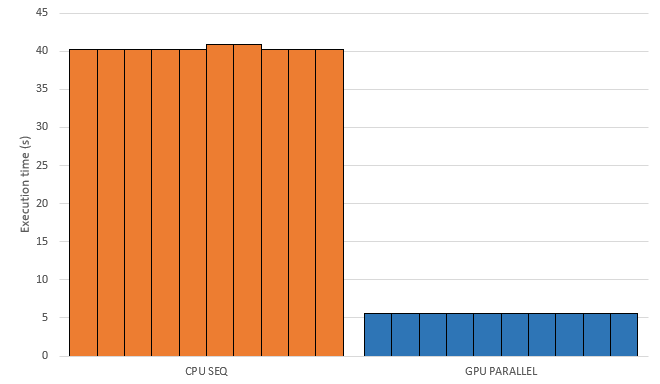
\includegraphics[width=\linewidth]{figures/graph_cpuVSgpupar.png}}
	\caption{Execution time of CPU sequencial vs GPU Parallel.}
	\label{fig1}
\end{figure}
\begin{figure}[htbp]
	\centerline{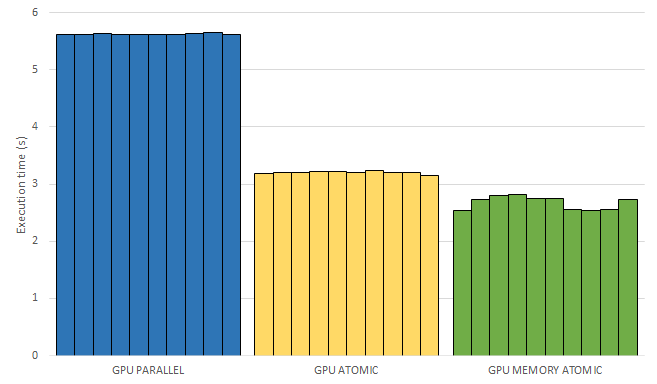
\includegraphics[width=\linewidth]{figures/graph_gpus.png}}
	\caption{Execution time of our gpu implementations.}
	\label{fig1}
\end{figure}

\subsection{Discussion}

With the results demonstrated, we can see the little improvements that can be made in GPGPU and how much impact they can make in performance of the kernel. It should be possible to understand why each of the improvements is needed and should be taken in consideration when using the GPU. The most significant change in all the parallel implementations would be the use of synchronization to avoid the recurrent call of the kernel to synchronize, in the Floyd Warshall in specific this recurrent call of kernels can add a big overhead since it relies massively on synchronization. That is why when using only one call due to the synchronization, the time taken decreased around 43\% which is the biggest improvement made. Then we could even improve this version by reducing the number of reads from global memory, this improvement alone decreased the time taken by around 16.5\%. This proves that each improvement in GPGPU can make a big difference, even more when working with bigger work sizes.

\begin{comment}
Here you should discuss the results on a high level. For instance, based on our results, the parallelization of the merge-sort is relevant as no other parallel work occurs at the same time, and the complexity $O(N log(N))$ can have a large impact when the number of individuals is high.
\end{comment}

\section{Related Work}

As we developed this paper, we found two papers that approached CUDA programing but both differed on the scope of the topic. \cite{floyd warshall}Analyzes the Floyd Warshall algorithm in detail but it does not provide a good introduction to GPGPU. \cite{study on FDTD}Provided a more in depth approach to CUDA, showing as well how it could be use to tackle FDTD, but again it lacks as a teaching tool toward people that aim to learn the basics of CUDA and GPGPU programing.

\section{Conclusions}

The goals of this paper is to provide a good teaching paper to those who want to start learning GPGPU, explaining from the basics, for example grid composition and memory allocation to the device, to the improvements that can be made to the use of memory. It is shown the impact of the improvements so that it can be interpreted the differences that those improvements make.
After all the results presented before, we can conclude that it is not always recommended to use GPGPU, but when the work load is big enough and something that can be parallelized, then it should be taken into consideration due to the fact that it can reduce significantly the time taken to compute such task. We can verify too that even though the performance can already be good when only converting to the most basic of parallel GPU programing, it should be taken advantage of the different refinements on the GPU such as the shared memory, registry memory and the synchronization between thread in a block. Each problem will take more or less advantage of each improvement but at the end, by doing them, the results should pay off.

\section*{Acknowledgements}

Regarding to the implementation of the code both authors worked on it, with the second author focusing more in the implementation details. Both authors authors wrote the paper, where the first author focused more on evaluation, related work, bibliography and in the detailing both the sequential versions, as well as the parallel GPU version. The second author focused more the introduction, abstract, conclusions and in the synchronization and memory improvement versions explanations.
All the formating of paper was done by the first author.

Each author spent around 40 hours on this project.

\bibliography{splncs04}

\begin{thebibliography}{00}
	\bibitem{memory} Harris, M. (2013, January 28). Using Shared Memory in CUDA C/C++. Retrieved January 15, 2020, from https://devblogs.nvidia.com/using-shared-memory-cuda-cc/
	\bibitem{occupancy} Achieved Occupancy. (2016, March 31). Retrieved January 22, 2020, from https://docs.nvidia.com/gameworks/content/developertools/desktop/
	/analysis/report/cudaexperiments/kernellevel/achievedoccupancy.htm
	\bibitem{programing guide} CUDA C++ Programing Guide. (2019, November 28). Retrieved December 20, 2019, from https://docs.nvidia.com/cuda/cuda-c-programming-guide/index.html
	\bibitem{best practices} CUDA C++ Best Practices Guide. (2019, November 28). Retrieved January 2, 2020, from https://docs.nvidia.com/cuda/cuda-c-best-practices-guide/index.html
	\bibitem{study on FDTD} Donno, D., \& Esposito, A., \& Tarricone, L., \& Catarinucci, L. (June 2010). Introduction to GPU Computing and CUDA Programming: A Case Study on FDTD. IEEE Antennas and Propagation Magazine, 52.  
	\bibitem{floyd warshall} Kulkarni, K., \& Sharma, N., \& Shinde, P., \& Varma, V. (January 2015). Parallelization of Shortest Path Finder on GPU:Floyd-Warshall. International Journal of Computer Applications, 110. 
\end{thebibliography}

\end{document}
